\documentclass[fullscreen=true, bookmarks=true, hyperref={pdfencoding=unicode}]{beamer}
\usepackage[utf8]{inputenc}                                % Кодировка
\usepackage[english,russian]{babel}                        % Переносы
\usepackage{xcolor}                                        % Работа с цветом
\usepackage{amsmath,amssymb,amsfonts}                      % Символы АМО
\usepackage{graphicx}                                      % Графика
\usepackage[labelsep=period]{caption}                      % Разделитель в подписях к рисункам и таблицам
\usepackage{hhline}                                        % Для верстки линий в таблицах
\usepackage{tikz}                                          % Для простых рисунков в документе
\usepackage{fancybox}                                      % Пакет для отрисовки рамок
\usepackage{verbatim}                                      % Для вставки кода в презентацию
\usepackage{animate}                                       % Для вставки видео в презентацию
\usepackage{xmpmulti}                                      % Для вставки gif в презентацию
\usepackage{multirow}

\usetikzlibrary{arrows,snakes,backgrounds}                 % Для отрисовки стрелок

\graphicspath{{images/}}                                   % Путь до рисунков
\setbeamertemplate{caption}[numbered]                      % Включение нумерации рисунков

\definecolor{links}{HTML}{2A1B81}                          % blue for url links
\hypersetup{colorlinks,linkcolor=,urlcolor=links}          % nothing for others

\usetheme{Boadilla}
\usecolortheme{whale}

\usepackage{minted}

% \setbeameroption{show notes}
\setbeameroption{hide notes}
% \setbeameroption{show only notes}

\title{Lecture 6. Convolutional Neural Networks}
\author{Alex Avdyushenko}
\institute{Kazakh-British Technical University}
\date{October 15, 2022}
\titlegraphic{
\includegraphics[keepaspectratio,width=0.4\textwidth]{logo_kbtu.png}}

\begin{document}
%\unitlength=2mm

% выводим заглавие
\begin{frame}
\transdissolve[duration=0.2]
\titlepage
\end{frame}

\note{Hello, today we are going to talk about Convolutional Neural Networks, their history and development.

And we will start with three questions for five minutes based on the materials of the previous lecture.}

\begin{frame}
  \frametitle{Five-minute questions}
  \pause
  \begin{itemize}
    \item What is Neuron in deep learning?
    \item What is ImageNet?
    \item Give some examples of activation functions.
  \end{itemize}

\note{Please, write answers or send photos with them directly to me in private messages here in Teams, so that others cannot read your message. Last time, a lot of people did it, so I believe that this time you all will succeed.}

\end{frame}


{ % all template changes are local to this group.
    \setbeamertemplate{navigation symbols}{}
    \begin{frame}<article:0>[plain]
        \begin{tikzpicture}[remember picture,overlay]
            \node[at=(current page.center)] {
                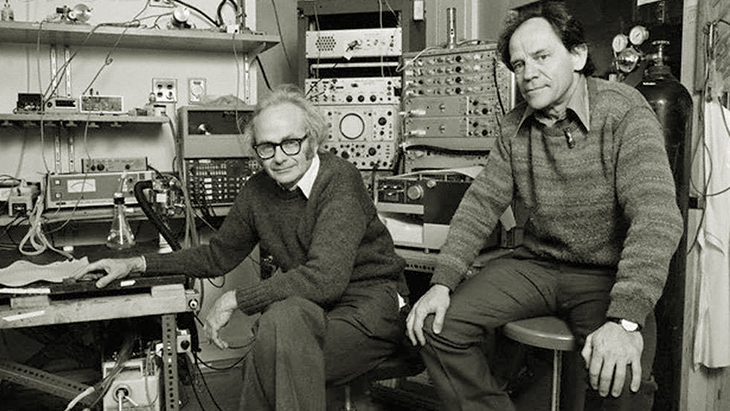
\includegraphics[keepaspectratio,
                                 width=\paperwidth,
                                 height=\paperheight]{img_EP_hubel-weisel-toys2.jpg}
            };
        \end{tikzpicture}
     \end{frame}
}

\note{Who is in this photo?

These are Hubel and Wiesel, Nobel Prize winners in Physiology or Medicine, who have explored the mechanisms of human vision.}

\begin{frame}
  \frametitle{Hubel \& Wiesel (1959)}
  \framesubtitle{History}
  The Nobel Prize in Physiology or Medicine, 1981
\end{frame}


{ % all template changes are local to this group.
    \setbeamertemplate{navigation symbols}{}
    \begin{frame}<article:0>[plain]
        \begin{tikzpicture}[remember picture,overlay]
            \node[at=(current page.center)] {
                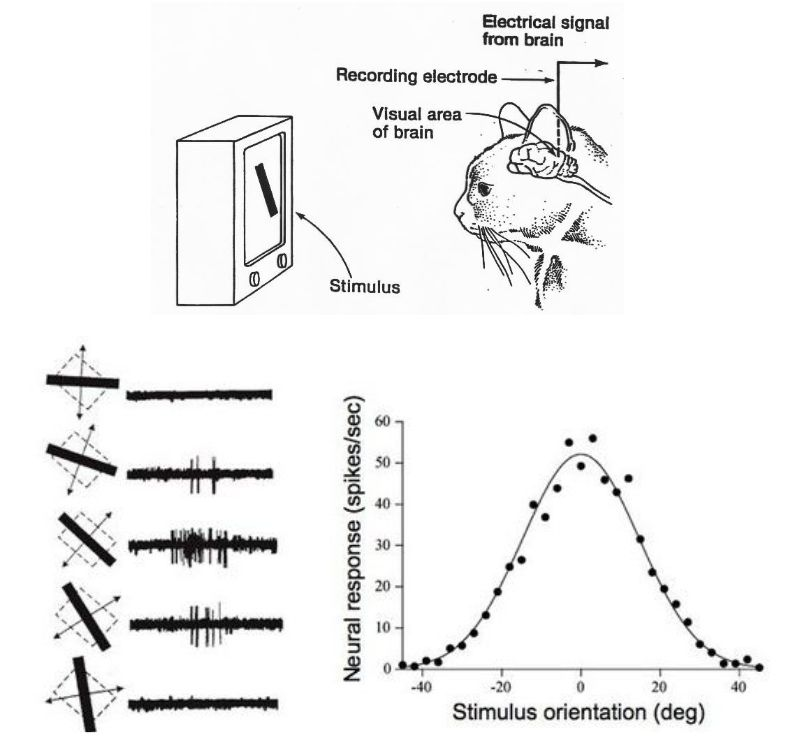
\includegraphics[keepaspectratio,
                                 width=\paperwidth,
                                 height=\paperheight]{cat_and_directions.jpeg}
            };
        \end{tikzpicture}
     \end{frame}
}

\note{In their most famous work, they showed a cat variously oriented black stripes and recorded the response of brain neurons.

And in fact, they discovered the neurons responsible for the angle of rotation of the strips.}

\begin{frame}
   \frametitle{Idea of hierarchical organization of vision}
   \framesubtitle{History}
  \begin{center}
    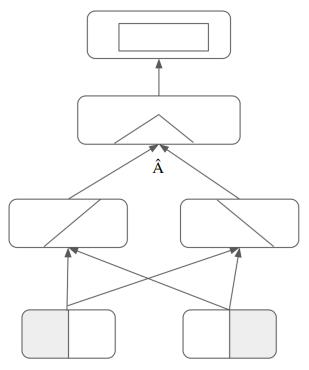
\includegraphics[keepaspectratio,
                     height=0.8\paperheight]{hierarchy_vision.jpg}
  \end{center}

  \note{Then, quite quickly, an understanding of the hierarchical organization of human vision came, which was confirmed by other works.

  That is, at first the neurons of the brain distinguish stripes, color gradients. The stripes form corners and further more and more complex elements: geometric shapes and so on up to abstract concepts.}
\end{frame}


\begin{frame}
  \frametitle{Fukushima (1980)}
  \framesubtitle{History}
  \begin{center}
    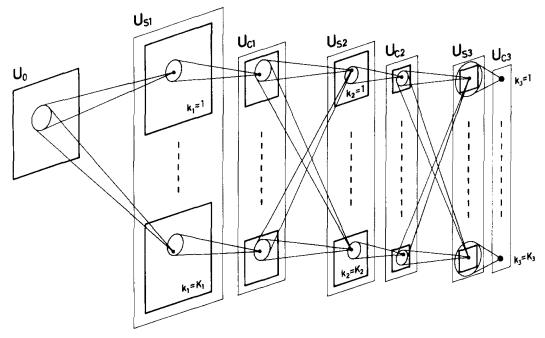
\includegraphics[keepaspectratio,
                     height=0.5\paperheight]{Fukushima_1980.png}
  \end{center}

  Convolutions and activations have already been used, but without gradient descent optimization and supervised learning

  \note{One of the very first neural networks for image analysis was organized in a similar way, but it has not been yet gradient descent optimization and supervised learning.}
\end{frame}


\begin{frame}
  \frametitle{Lekun, Bottou, Bengio, Haffner (1998)}
  \framesubtitle{First success}
  \begin{center}
    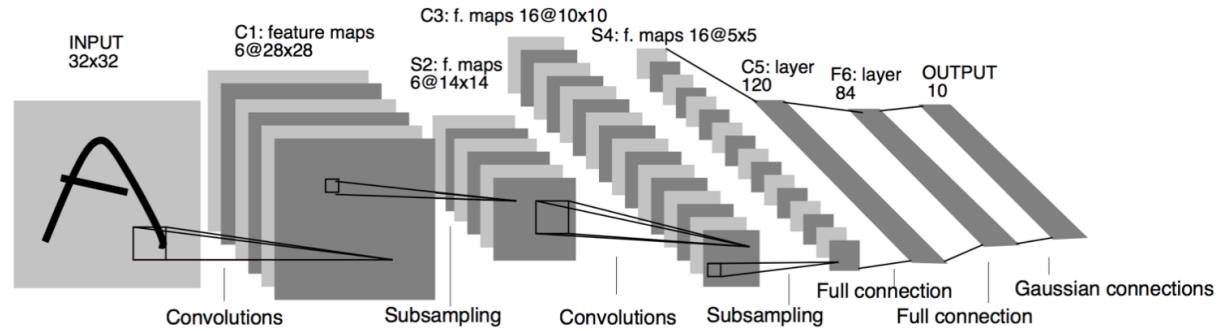
\includegraphics[keepaspectratio,
                     height=0.33\paperheight]{LeNet.jpg}
  \end{center}

  \note{Then quite good results were obtained using the LeNet architecture.}

\end{frame}


\begin{frame}
  \frametitle{Krizhevsky, Sutskever, Hinton (2012)}
    \framesubtitle{A real breakthrough}
    The Winner of the ImageNet contest of the 2012 year
  \begin{center}
    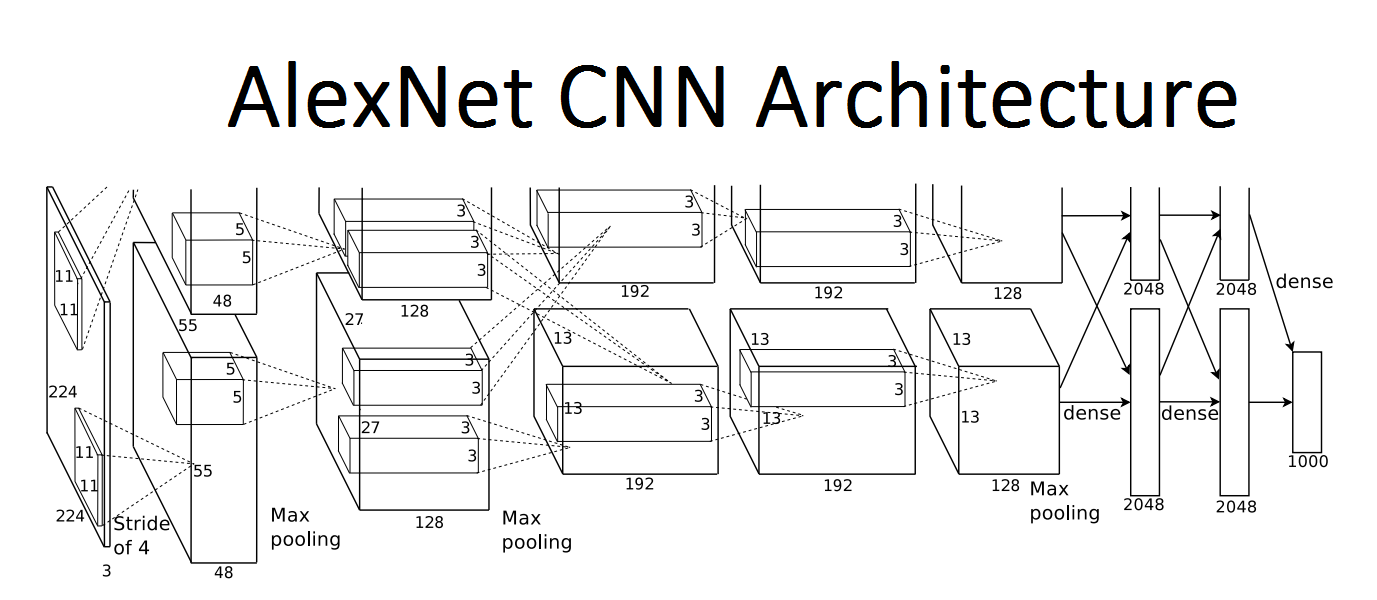
\includegraphics[keepaspectratio,
                     height=0.5\paperheight]{AlexNetCNN.png}
  \end{center}

  \note{And the first real breakthrough in image classification was made by AlexNet neural network.}

\end{frame}


\begin{frame}
  \frametitle{Linear model}
  \framesubtitle{Recall}

 $x^1, x^2, \dots, x^n \in \mathbb{R}$ — numerical features of one object $x$
 
 $w_0, w_1, \dots, w_n \in \mathbb{R}$ — weights of features
 
 $$a(x, w) = \sigma(\left<w, x\right>) = \sigma \left(\sum\limits_{j=1}^n w_j f_j(x) - w_0 \right),$$
 
 $\sigma(z)$ — activation function, for example one of the:
 $\text{sign}(z),\ \frac{1}{1+e^{-z}},\ (z)_+$

\begin{center}
  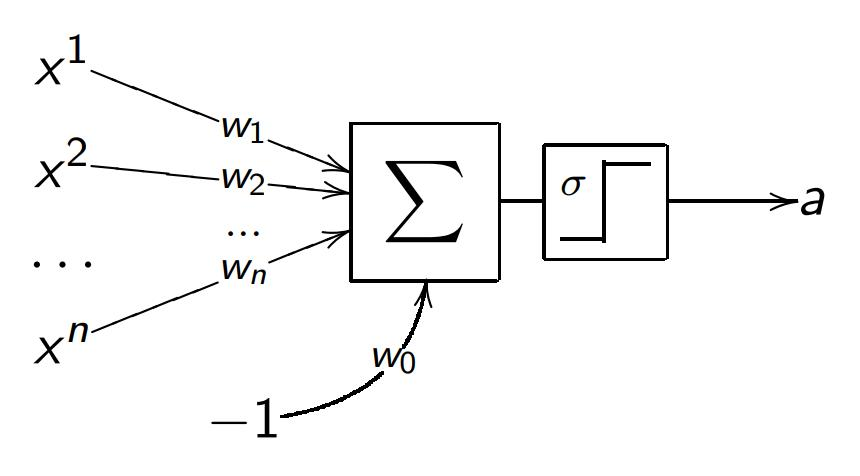
\includegraphics[keepaspectratio, width=.5\paperwidth]{lin_as_nn.jpg}
\end{center}

\note{Let's recall the linear model from the last lecture: numerical features only, their weights and one simple activation function. That's it!}

\end{frame}


\begin{frame}
  \frametitle{Neural network as a combination of linear models}
  \begin{center}
    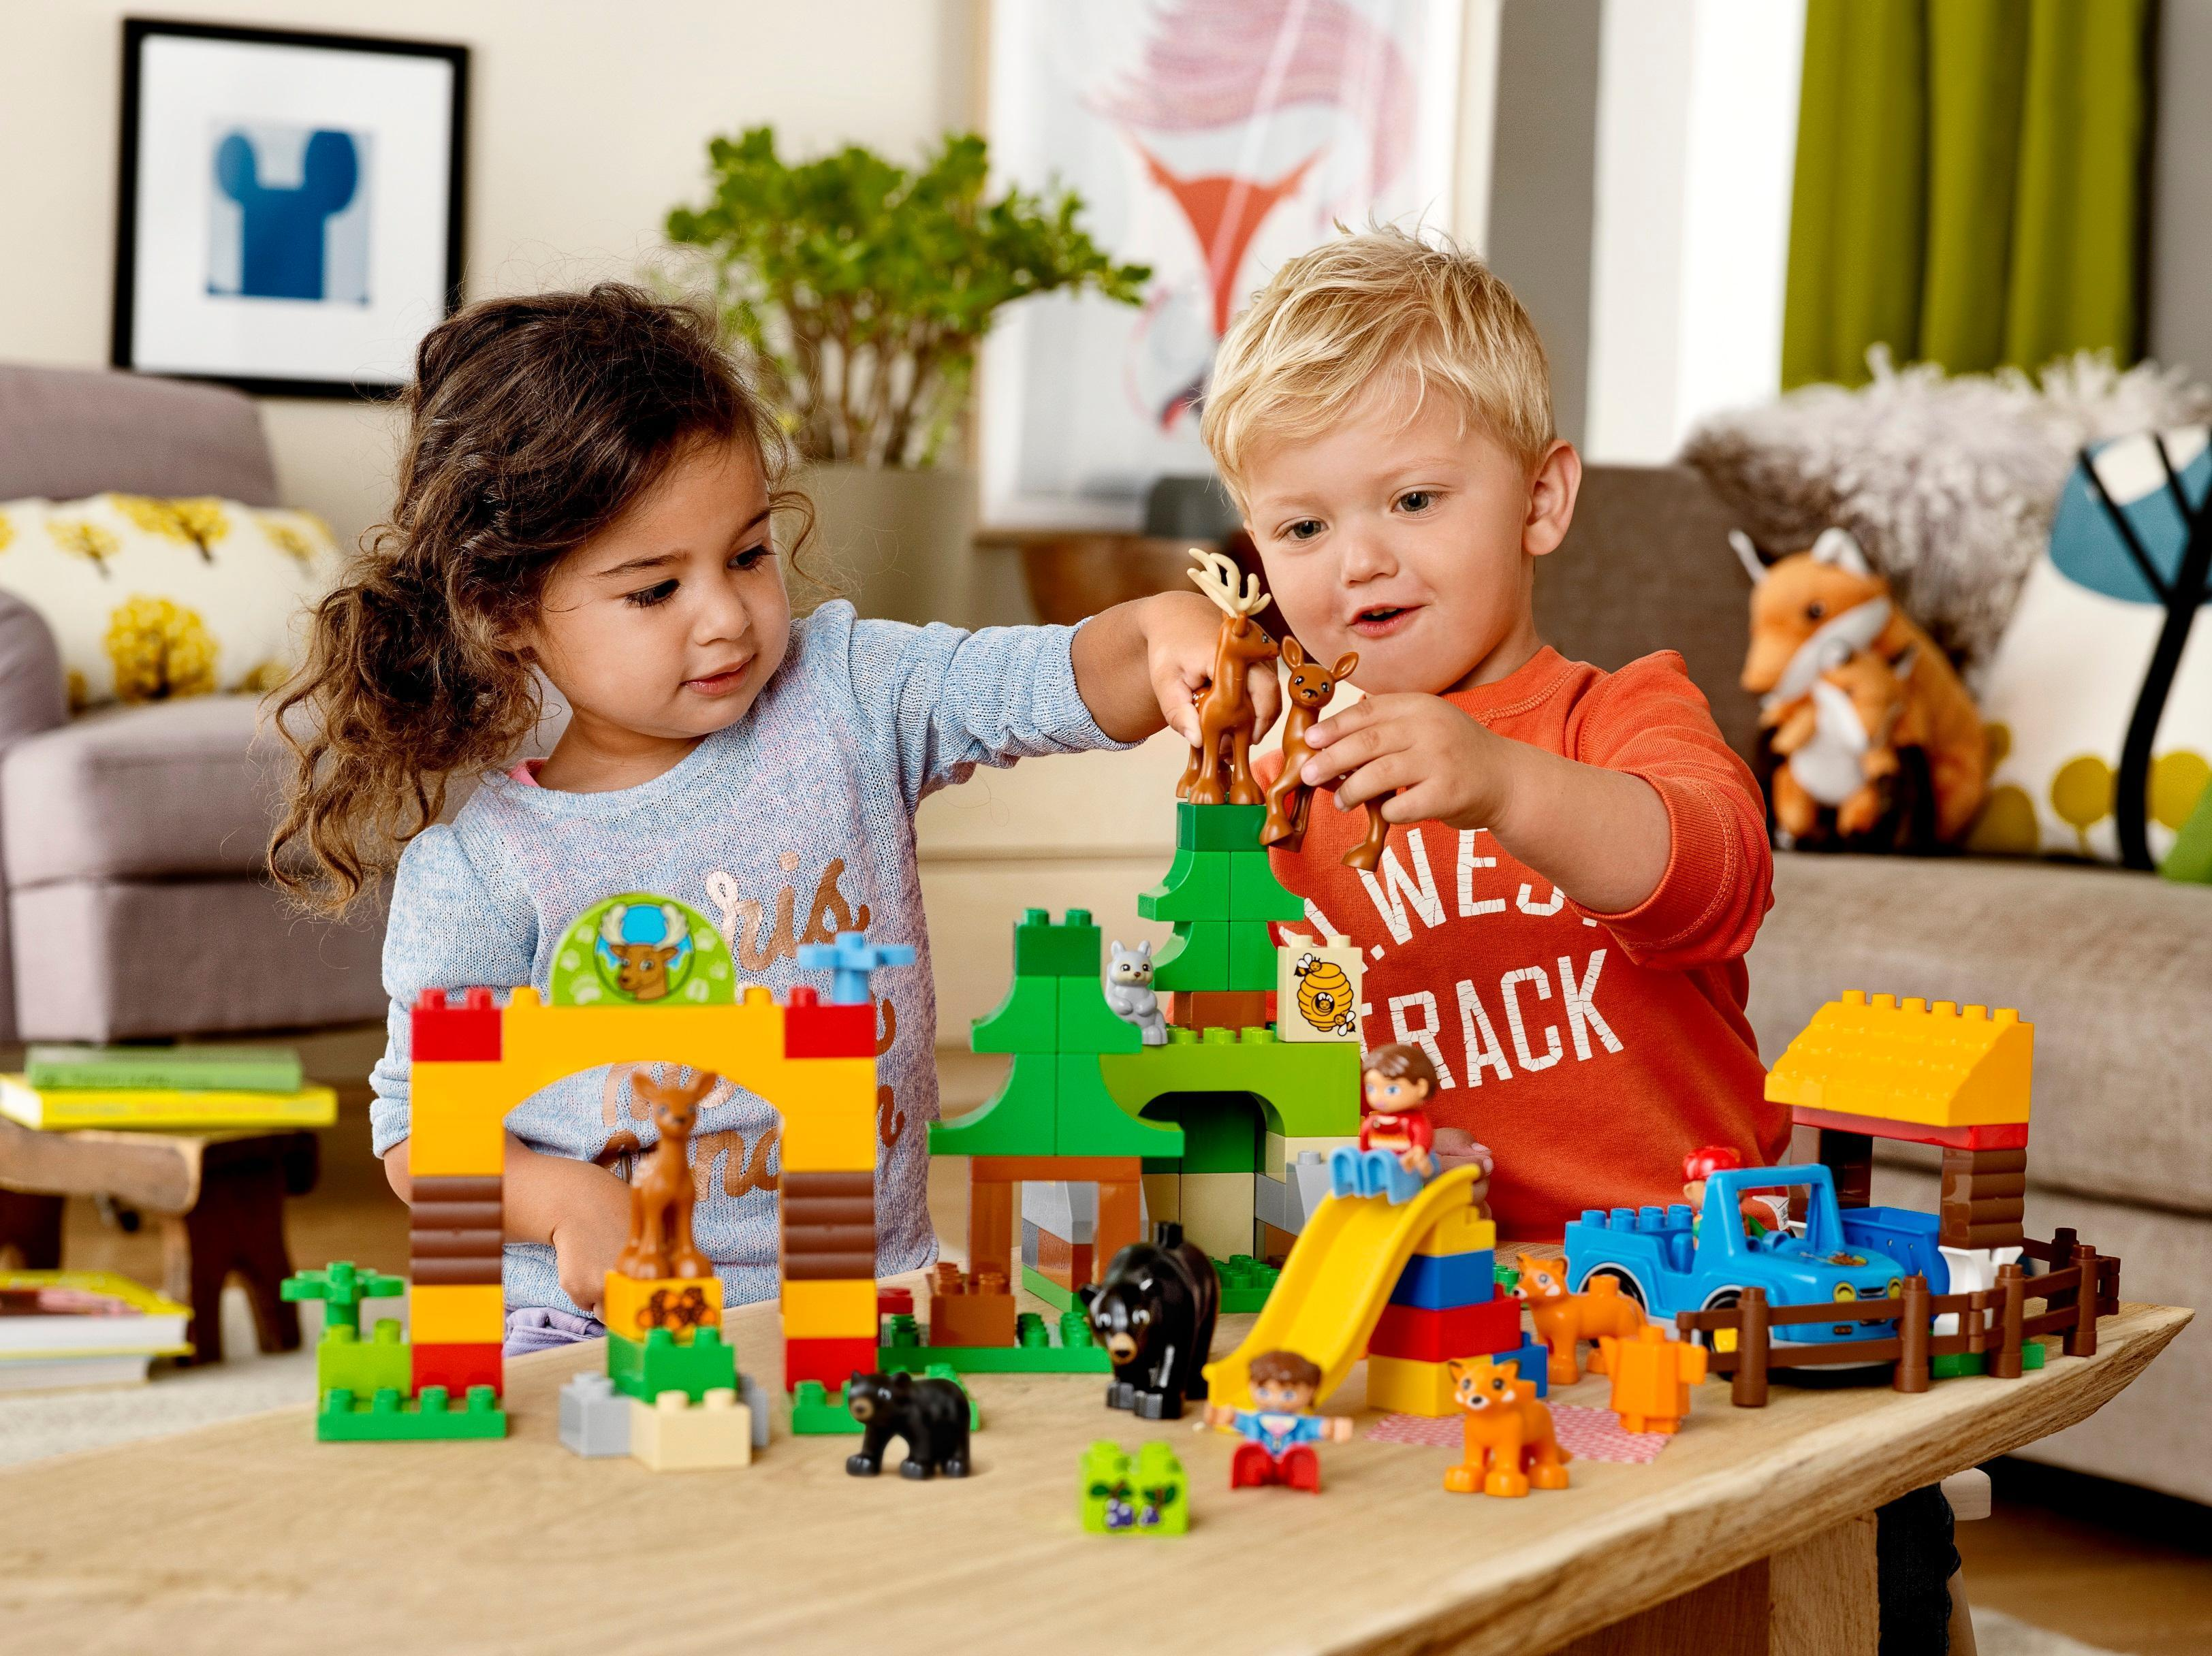
\includegraphics[keepaspectratio,
                     height=0.8\paperheight]{nn-as-lego-duplo.jpg}
  \end{center}

  \note{And neural network in essence is a combination of linear models}
\end{frame}


\begin{frame}
  \frametitle{Convolutional Neural Network}
  \begin{center}
    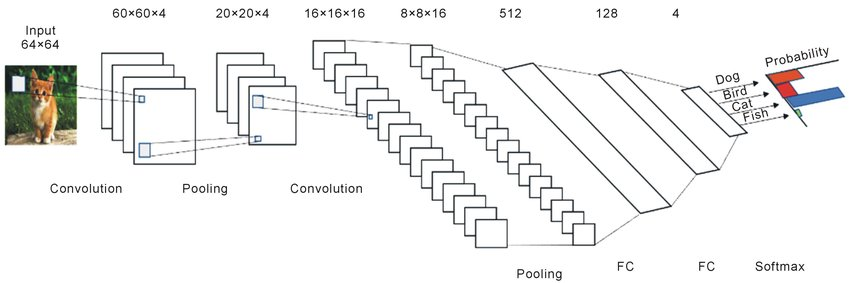
\includegraphics[keepaspectratio,
                     width=0.9\paperwidth]{cnn-example.png}
  \end{center}

  \note{Ok, and what is Convolutional Neural Network? This is a fairly natural development of the model. In addition to the fully connected layer already familiar to us, there are also convolutional layers and pooling layers.}

\end{frame}


\begin{frame}
\frametitle{Convolution}
   Convolution in neural networks — the sum of products of elements
  \begin{itemize}
    \item radical reudce of training parameters $28^2 = 784 \to 9 = 3^2$ to get the same accuracy
    \item Directions $x$ and $y$ are built into the model
  \end{itemize}


  \begin{center}
    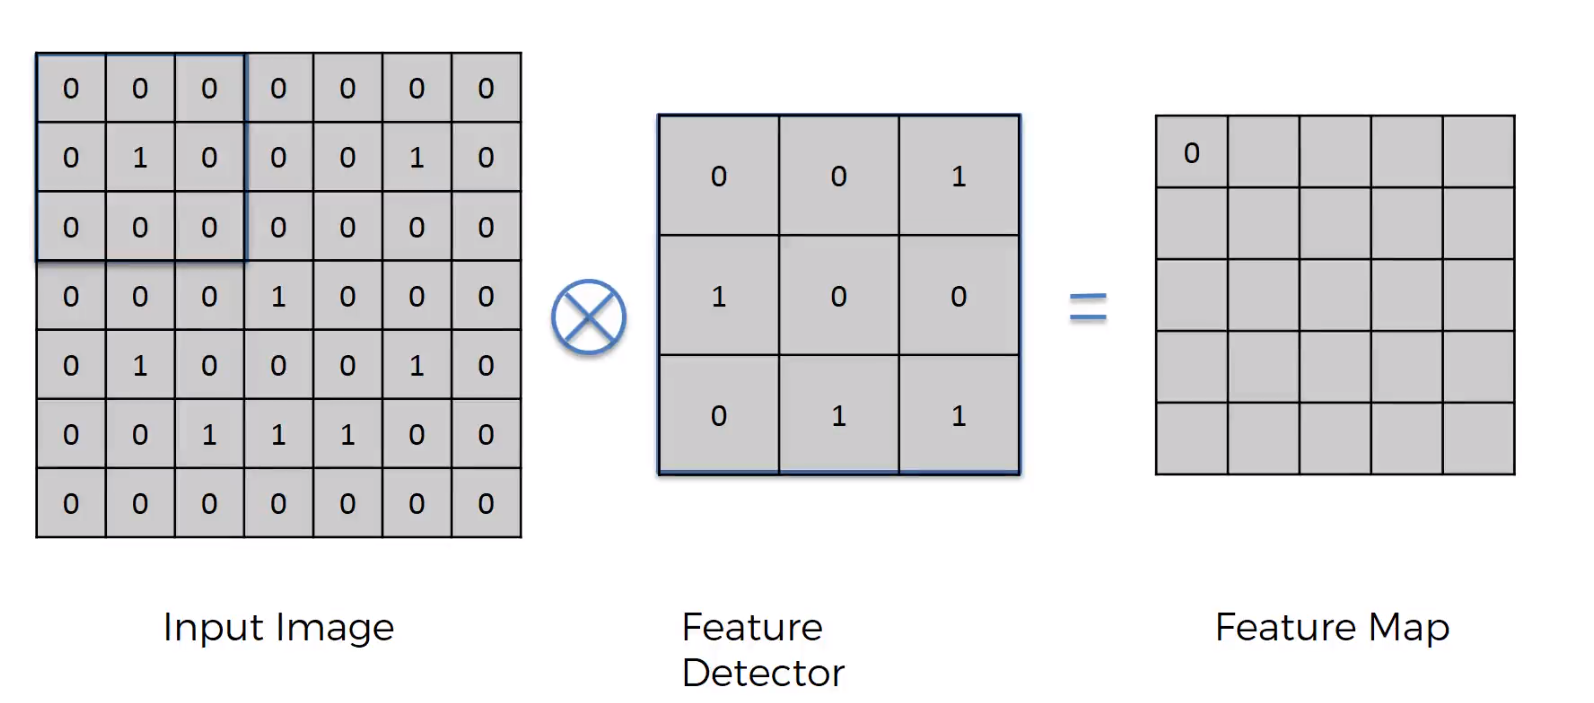
\includegraphics[keepaspectratio,
                     width=0.8\paperwidth]{conv-example.png}
  \end{center}

  \note{The convolutional layer allows you to get the same result many times more efficiently than the fully connected layer.

  Moreover, through it, two selected directions x and y are built into the model, which are really physically important for understanding the image.}

\end{frame}


\begin{frame}
    \begin{block}{Question 1}
    Why is it called <<сonvolution>>?
    \end{block}
    \pause
    \begin{alertblock}{Note}
    The implementation of convolution effectively multiplies a matrix by a vector. Here, for example, \href{https://arxiv.org/pdf/1509.09308.pdf}{an article with the implementation of Winograd transformation} in cuDNN.
    \end{alertblock}
\end{frame}


\begin{frame}
  \frametitle{Convolution operation example}
   Kernel $3\times3\times3$ (Width $\times$ Height $\times$ Channel numbers)  
  \begin{center}
    \animategraphics[loop,width=0.8\paperwidth,autoplay]{1}{conv_live-}{0}{7}
  \end{center}

  \note{Let's look at example of convolution operation. It is important to notice, that bias is one value}

\end{frame}


\begin{frame}
  \frametitle{Padding and stride}
  \begin{center}
    \animategraphics[loop,width=0.9\paperwidth,autoplay]{8}{padding_and_stride-}{0}{67}
  \end{center}
\end{frame}

\begin{frame}
  \frametitle{Dilation (=2)}
  \begin{center}
    \animategraphics[loop,width=0.5\paperwidth,autoplay]{1}{dilation-}{0}{8}
  \end{center}
\end{frame}


\begin{frame}
  \frametitle{Calculate the size of the output}
  \begin{itemize}
    \item {\bf F}ilter size = 3$\times$3 $\to$ 3
    \item {\bf I}nput size = 28$\times$28 $\to$ 28
    \item {\bf S}tride = 1x1 $\to$ 1
    \item {\bf P}adding = 0x0 $\to$ 0
  \end{itemize}

  Output size = (I - F + 2*P)/S + 1 = (28 - 3 + 2*0)/1 + 1 = 26

  Output size = 26 $\to 26\times 26$

  \note{Imagine that we need to calculate the size of the output of the convolution layer. Now we can easily understand why the formula is exactly that}
\end{frame}


\begin{frame}
  \frametitle{Pooling}
  \begin{center}
    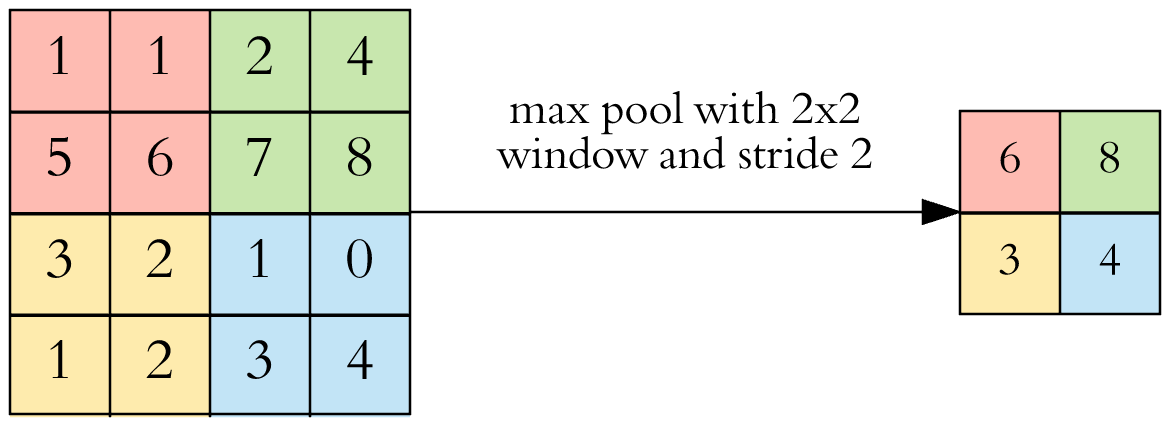
\includegraphics[keepaspectratio,
                     width=0.8\paperwidth]{max_pooling.png}
  \end{center}

  \note{Pooling layer is maybe the simplest layer of all: we choose the maximum element of filter. Or there is average pooling, where we take mean, but it is used quite rarely}

\end{frame}


\begin{frame}
\frametitle{Sigmoid Activation Functions}
  \framesubtitle{Recall}
   \begin{itemize}
     \item Logistic sigmoid
     $\sigma(z) = \frac{1}{1+\exp(-z)}$

     \pause
     \item Hyperbolic tangent
     $\tanh(z) = \frac{\exp(z)-\exp(-z)}{\exp(z)+\exp(-z)}$

     \pause
     \item continuous approximations of threshold function
     
     \pause
     \item can lead to vanishing gradient problem and "paralysis" of the network
   \end{itemize}

  \pause
  \begin{block}{Question 2}
  What are the disadvantages of the logistic sigmoid?
  \end{block}
\end{frame}


\begin{frame}
  \frametitle{Let's look at the charts again}
  \begin{center}
    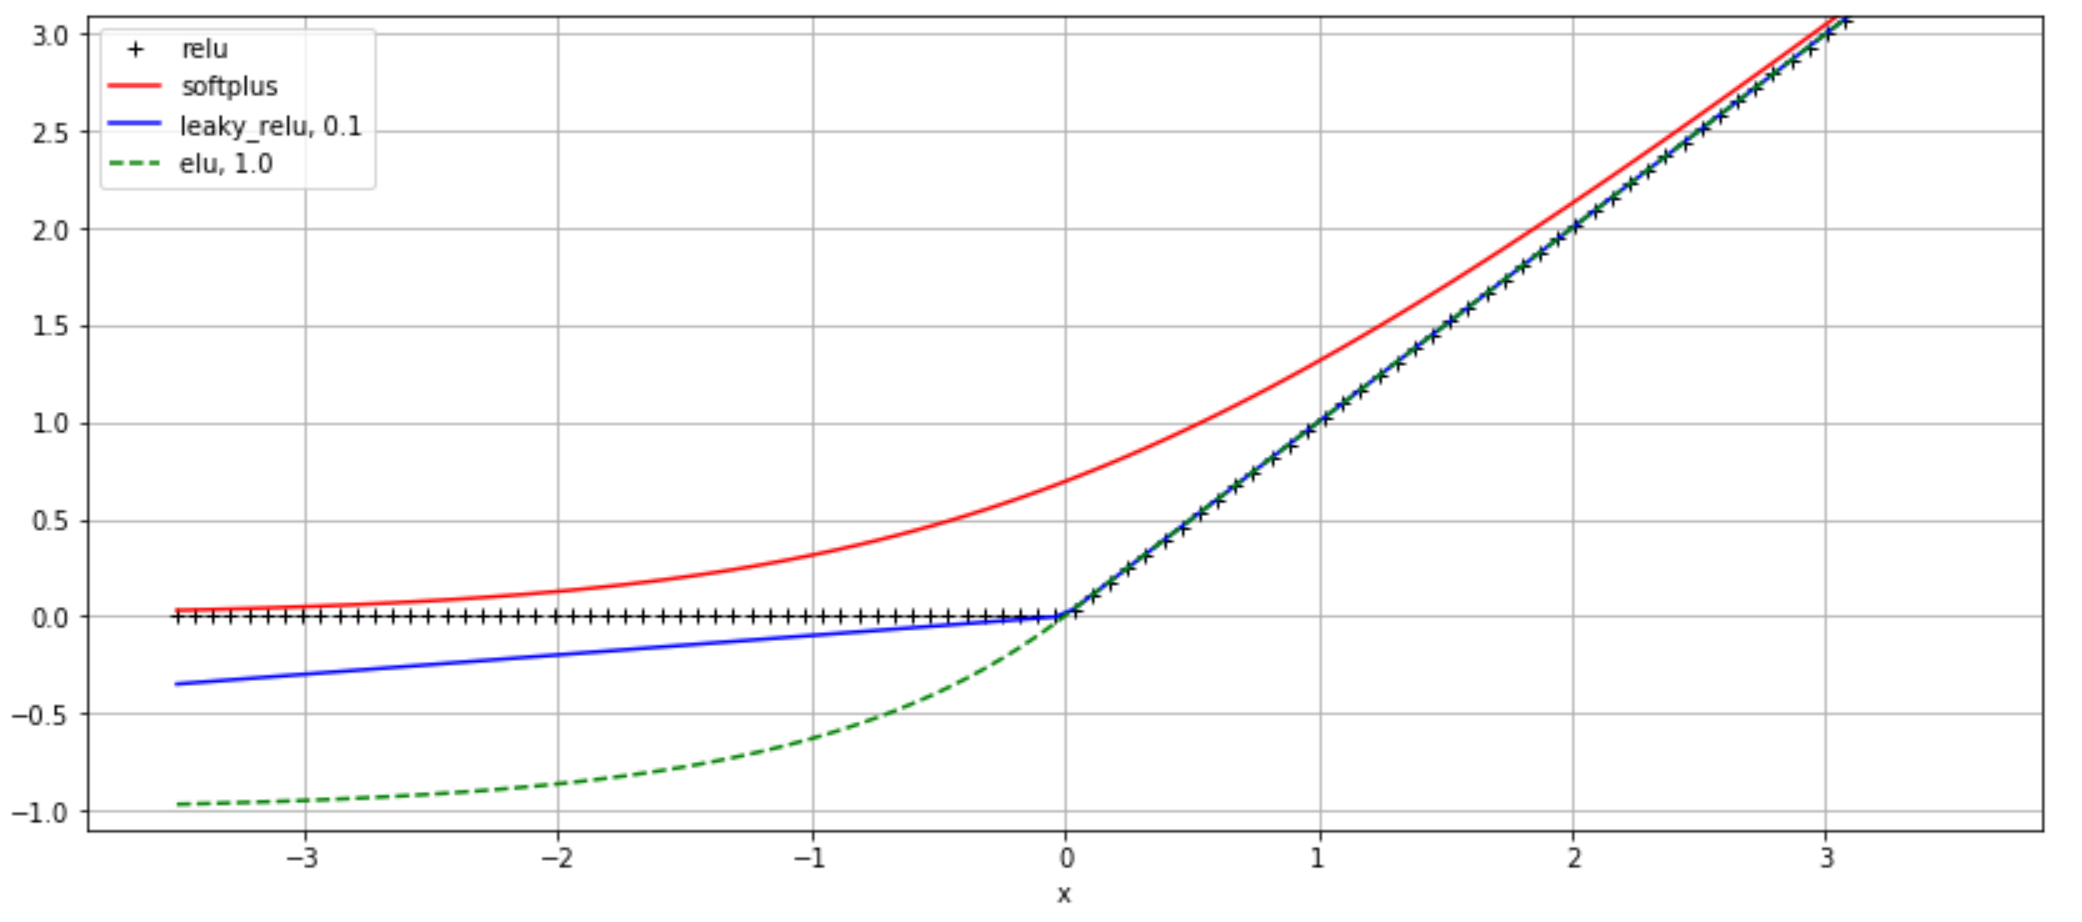
\includegraphics[keepaspectratio,
                     width=0.9\paperwidth]{relu_softplus.png}
  \end{center}

  \note{The main disadvantage of sigmoid is that it's derivateve is close to zero for arguments greater than 3. So your default choice is ReLU, than you could try LeakyReLU and softplus.}

\end{frame}


\begin{frame}
  \frametitle{The progress of convolutional networks}
  \framesubtitle{Or a brief history of ImageNet}

  \begin{center}
    \begin{tikzpicture}
        \node[anchor=south west,inner sep=0] at (0,0) {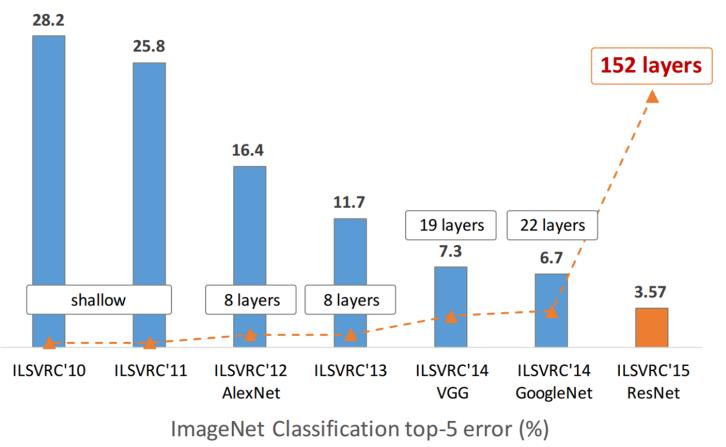
\includegraphics[keepaspectratio, height=0.7\paperheight]{image-net-history.jpg}};
        \draw<2>[red,ultra thick,rounded corners] (3.0,0.5) rectangle (4.55,5.0);
    \end{tikzpicture}

    \note{We have seen the remarkable progress in solving the problem of image classification
of ImageNet collection. Now let's dive into the details of the AlexNet architecture.}

\end{center}

\end{frame}


\begin{frame}
  \frametitle{AlexNet (Krizhevsky, Sutskever, Hinton, 2012)}
  \framesubtitle{The Winner of the ImageNet contest of the 2012 year}
  \begin{center}
    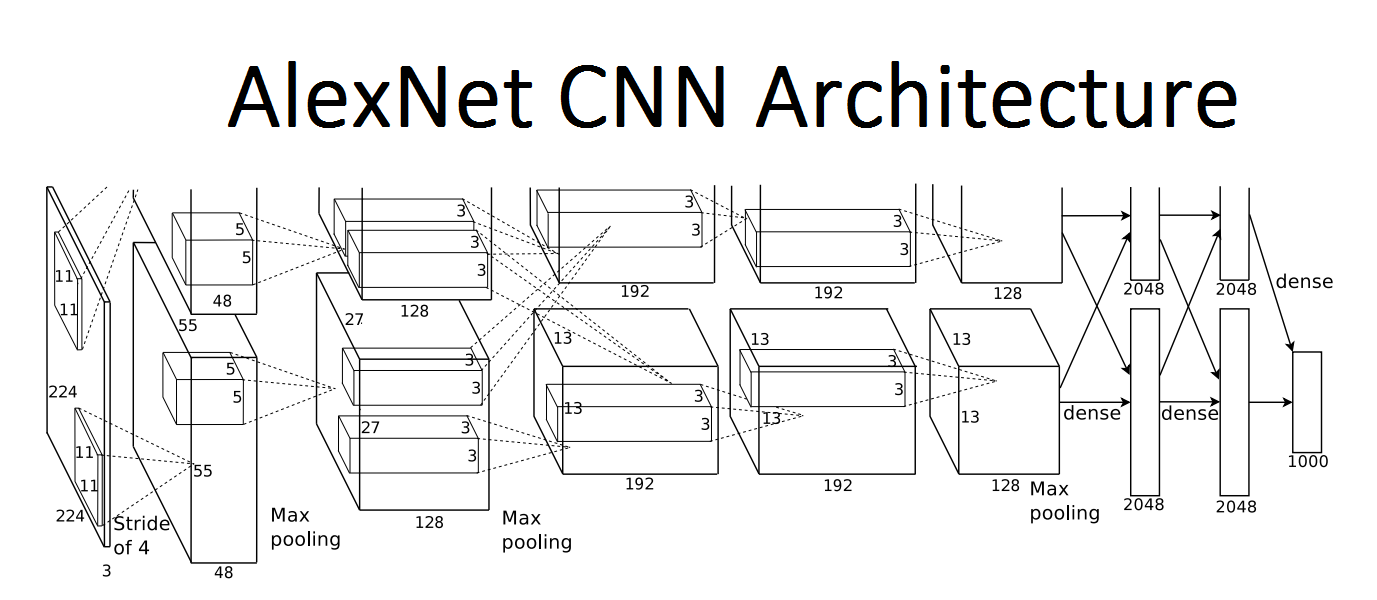
\includegraphics[keepaspectratio,
                     width=0.7\paperwidth]{AlexNetCNN.png}
  \end{center}
  \begin{itemize}
     \small
     \pause \item ReLU activation
     \pause \item L2 regularization 5e-4
     \pause \item {\it data augmentation}
     \pause \item {\it dropout 0.5}
     \pause \item {\it batch normalization} (batch size 128)
     \pause \item SGD Momentum 0.9
     \pause \item Learning rate 1e-2, then decrease by 10 times after quality stabilization on the test. Top5 final accuracy on ImageNet — 25.8\% $\to$16.4\%
   \end{itemize}

\end{frame}


\begin{frame}
\frametitle{Momentum method}

   \begin{columns}
     \begin{column}{0.45\paperwidth}
     Momentum accumulation method [B.T.Polyak, 1964] — exponential moving average of the gradient over $\frac{1}{1-\gamma}$ last iterations:

     $$\nu = {\color{red}\gamma} \nu + {\color{red}(1-\gamma)} \mathcal{L}_i^\prime(w)$$
     
     $$w = w - \eta \nu$$
     \end{column}
     \begin{column}{0.45\paperwidth}
     \centering
     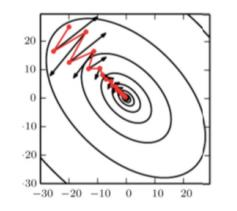
\includegraphics[keepaspectratio,
                      width=0.3\paperwidth]{momentum_2.jpg}
     \end{column}
   \end{columns}

   \note{A very popular method for improving the convergence of SGD is the momentum accumulation method. In it, from a physical point of view, the derivative of the loss function becomes the acceleration of the change in model parameters, and not the speed as in classical SGD.}

\end{frame}


\begin{frame}
\frametitle{Nesterov Accelerated Gradient (NAG, 1983)}

   \begin{columns}
     \begin{column}{0.45\paperwidth}
     $\nu = \gamma \nu + (1 - \gamma) \mathcal{L}_i^\prime (w - {\color{red}\eta \gamma v})$

     $w = w - \eta \nu$
     \end{column}
     \begin{column}{0.45\paperwidth}
     \centering
     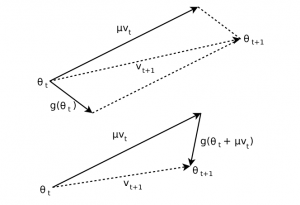
\includegraphics[keepaspectratio, width=0.3\paperwidth]{nag_vs_mom.png}
     
     {\small (Top) Momentum method

     (Bottom) Nesterov Accelerated Gradient

     $\mu$ is the decaying parameter, same as $\eta$}
     \end{column}
   \end{columns}

   \note{And one more small, but important improvement of the NAG method is to take the value of the derivative of the loss function at a future (next) point, and not at the current one.}

\end{frame}


\begin{frame}
  \frametitle{Summary}
  \begin{itemize}
    \item Convolutional networks are very well suited for image processing
    \item They are a bit like similar to biological vision mechanisms
    \item At the same time, flexible and computationally efficient
    \item Today, the <<de facto>> standard for computer vision tasks (classification, detection, segmentation, generation)
    \pause
    \item Will be next
      \begin{itemize}
        \item various optimization algorithms: adam, RMSProp
        \item dropout
        \item choice of initial approximation
        \item ResNet and WideResNet
      \end{itemize}
  \end{itemize}

  \pause
  What else can you watch?
  \begin{itemize}
    \item \href{https://cs.stanford.edu/people/karpathy/convnetjs/}{Demo by Andrey Karpaty}
    \item There is a famous course from Stanford <<CS231n: Convolutional Neural Networks for Visual Recognition>>: \href{http://cs231n.github.io/}{http://cs231n.github.io/}
  \end{itemize}
\end{frame}
\end{document}
